%% 05_model1_stranded_assets.tex
%% Section 5: Model 1 -- Stranded Asset Valuation

\section{Model 1: Stranded Asset Valuation}
\label{sec:model1}

The first component of our framework quantifies the firm-level distribution of stranded asset values across Indonesia's coal sector. We employ three complementary analytical tools: a supply cost curve that visualises which firms become uneconomic under different price scenarios, a scenario-contingent discounted cash flow (DCF) model that produces net present values (NPVs) under alternative climate pathways, and a Monte Carlo simulation that quantifies uncertainty around these estimates.

\subsection{Supply Cost Curve}
\label{subsec:supply_cost}

We construct an industry supply cost curve by ranking the 15 coal companies for which we have both verified production data and cost of revenue data by their all-in breakeven price, defined as the minimum coal price at which the company's extraction operations generate non-negative cash flows. Formally, the breakeven price for firm $i$ is:
\begin{equation}
\label{eq:breakeven}
P_i^{BE} = C_i^{cash} + C_i^{royalty} + C_i^{transport} + C_i^{SGA} + r_i \cdot K_i / Q_i
\end{equation}
where $C_i^{cash}$ is the cash extraction cost per tonne, $C_i^{royalty}$ represents government royalty obligations, $C_i^{transport}$ captures transport and logistics costs, $C_i^{SGA}$ accounts for selling, general, and administrative expenses, $r_i$ is the required return on invested capital, $K_i$ is capital employed, and $Q_i$ is annual production volume.

The supply cost curve plots cumulative annual production on the horizontal axis against breakeven price on the vertical axis, producing a step function where each step represents an individual firm's production volume at its cost of extraction. Overlaying scenario-specific price lines (\$120/t for BAU, \$90/t for the 2\textdegree C pathway, and \$70/t for the 1.5\textdegree C pathway at the 2030 horizon) immediately identifies which firms become uneconomic under each scenario.

Figure~\ref{fig:supply_cost} presents the supply cost curve for the 15 firms with verified production and cost data, representing 390~Mt of annual output. Several features are noteworthy. First, the cost distribution is highly dispersed, with breakeven prices ranging from \$21.9/t for the lowest-cost producer (BUMI, which benefits from large-scale operations at KPC and Arutmin) to \$151.1/t for smaller operators with higher cost structures (HRUM). Second, under the 2\textdegree C scenario price of \$90/t at 2030, firms representing approximately 7\% of the sample's production become uneconomic (ITMG, TOBA, and HRUM, with a combined 27~Mt). Under the 1.5\textdegree C price of \$70/t, this share rises to approximately 15\%, adding INDY and MBAP to the uneconomic group.

\begin{figure}[htbp]
\centering
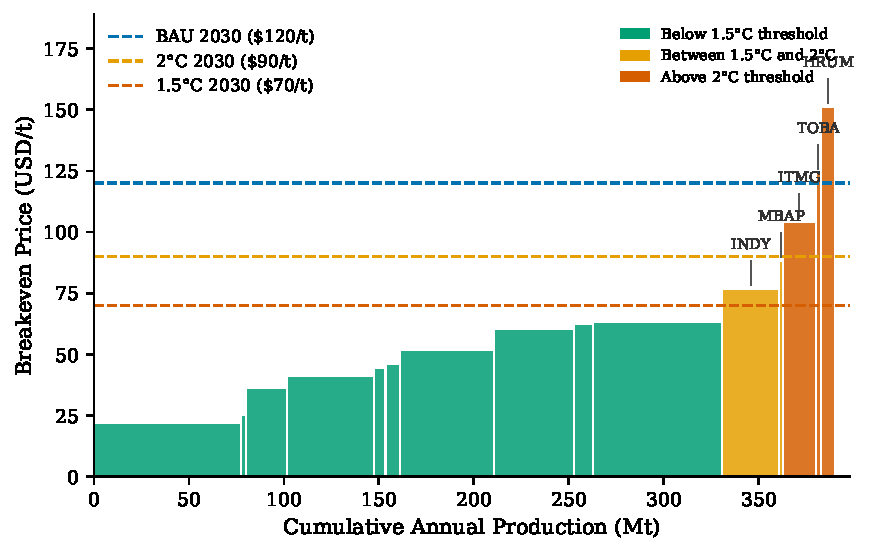
\includegraphics[width=\textwidth]{figures/fig_02.pdf}
\caption{Supply cost curve for Indonesian listed coal companies. Each step represents a single firm, with width proportional to annual production (Mt) and height equal to the all-in breakeven price (USD/t). Horizontal dashed lines indicate 2030 coal prices under three climate scenarios. Firms above a scenario line become uneconomic under that pathway.}
\label{fig:supply_cost}
\end{figure}

\subsection{Scenario-Contingent Net Present Value}
\label{subsec:scenario_npv}

To translate the supply cost curve into dollar-valued stranded asset estimates, we compute the net present value of each firm's coal operations under three climate scenarios. For firm $i$ under scenario $s \in \{BAU, 2C, 1.5C\}$, the NPV is:
\begin{equation}
\label{eq:npv}
NPV_i^s = \sum_{t=1}^{T_i} \frac{Q_{i,t}^s \cdot (P_t^s - C_{i,t}) - \tau \cdot \max(0, Q_{i,t}^s \cdot P_t^s - C_{i,t} \cdot Q_{i,t}^s)}{(1 + r_i^s)^t}
\end{equation}
where $Q_{i,t}^s$ is firm $i$'s production in year $t$ under scenario $s$, $P_t^s$ is the coal price path under scenario $s$, $C_{i,t}$ is the all-in unit cost of production (assumed to grow at 2\% annually for cost inflation), $\tau = 0.22$ is the Indonesian corporate tax rate, $r_i^s$ is the discount rate (WACC plus a scenario-specific stranding risk premium), and $T_i$ is the remaining mine life in years.

The coal price paths are calibrated to the IEA World Energy Outlook scenarios \citep{IEA2023} and NGFS reference scenarios \citep{NGFS2022}. Under BAU, prices decline gradually from current levels of approximately \$120/t to \$85/t by 2050, reflecting secular but modest demand erosion. Under the 2\textdegree C Paris-aligned scenario, prices fall to \$90/t by 2030 and \$35/t by 2050, driven by accelerating renewable deployment and carbon pricing. Under the 1.5\textdegree C net-zero scenario, prices drop sharply to \$70/t by 2030 and \$15/t by 2050, reflecting rapid coal phase-out consistent with the IEA Net Zero Emissions pathway. Table~\ref{tab:scenarios} presents the full set of scenario parameters.

\begin{table}[htbp]
\centering
\caption{Scenario Parameters}
\label{tab:scenarios}
\footnotesize
\begin{tabular}{lccc}
\toprule
Parameter & BAU & 2\textdegree{}C Paris & 1.5\textdegree{}C NZE \\
\midrule
Coal price, 2030 (USD/t) & \$120 & \$90 & \$70 \\
Coal price, 2050 (USD/t) & \$85 & \$35 & \$15 \\
Carbon price, 2030 (USD/tCO\textsubscript{2}) & \$10 & \$50 & \$130 \\
Carbon price, 2050 (USD/tCO\textsubscript{2}) & \$25 & \$140 & \$250 \\
Demand reduction, 2030--2050 & Moderate & Significant & Severe \\
Probability weight & 30\% & 40\% & 30\% \\
\bottomrule
\end{tabular}

\smallskip
\noindent \textit{Notes:} Scenario parameters calibrated from IEA World Energy Outlook (2023) and NGFS Phase IV scenarios. Coal prices are thermal coal FOB Indonesia (6,322 kcal/kg GAR equivalent). Carbon prices reflect emerging Indonesian carbon pricing mechanisms scaled to global benchmarks. Probability weights reflect a Bayesian prior over policy trajectories.
\end{table}


The stranded value for firm $i$ under scenario $s$ is defined as the difference between the BAU and scenario-specific NPVs:
\begin{equation}
\label{eq:sv}
SV_i^s = NPV_i^{BAU} - NPV_i^s
\end{equation}

A firm is classified as ``stranded'' when $NPV_i^s < 0$, indicating that the present value of its coal operations is negative; that is, the firm would be better off ceasing extraction immediately. The expected stranded value, incorporating probability weights across scenarios, is:
\begin{equation}
\label{eq:expected_sv}
E[SV_i] = \sum_{s} \pi_s \cdot SV_i^s
\end{equation}
where $\pi_{BAU} = 0.30$, $\pi_{2C} = 0.40$, and $\pi_{1.5C} = 0.30$, reflecting the authors' assessment of scenario likelihoods informed by NGFS reference pathways \citep{NGFS2022}. The 2\textdegree C scenario receives the highest weight because it approximates the median policy outcome consistent with current NDC trajectories. The Dirichlet(3,4,3) sampling in our Monte Carlo simulation captures uncertainty around these weights, and the tornado sensitivity analysis (Section~\ref{subsec:robustness}) confirms that results are robust to alternative probability assignments.



\subsection{Results}
\label{subsec:model1_results}

\subsubsection{Firm-Level Stranded Values}

Table~\ref{tab:firm_sv} presents firm-level stranded asset results for the 15 companies with verified production and cost data, ranked by expected stranded value. Three patterns emerge.

First, stranding risk is highly concentrated. The top five companies, Bayan Resources (BYAN), Adaro Andalan Indonesia (AADI), Bumi Resources (BUMI), Bukit Asam (PTBA), and Golden Energy Mines (GEMS), account for over 75\% of the aggregate stranded value under both the 2\textdegree C and 1.5\textdegree C scenarios. This concentration reflects the dominance of large-scale producers in Indonesia's coal sector, where the top five firms control the majority of total listed production.

Second, the stranding threshold varies markedly with firm cost structure. Under the 2\textdegree C scenario, firms with breakeven prices above approximately \$90/t experience negative NPVs, while under the 1.5\textdegree C scenario, this threshold drops to roughly \$70/t. Higher-cost producers such as HRUM (breakeven \$151.1/t) and TOBA (\$124.1/t) face negative NPVs even under moderate transition pathways. In contrast, low-cost producers like BUMI (\$21.9/t) and BYAN (\$51.6/t) remain viable under 2\textdegree C but face substantial value erosion under 1.5\textdegree C.

Third, the stranded value as a fraction of total assets provides a more meaningful measure of firm vulnerability than the absolute dollar amount. Several mid-tier producers have stranded values exceeding 100\% of their book assets under the 1.5\textdegree C scenario, indicating that the economic loss from stranding exceeds the firm's entire asset base, a result driven by the capitalised value of future production embedded in reserve valuations but not fully reflected in accounting book values

\begin{landscape}
\begin{table}[htbp]
\centering
\caption{Firm-Level Stranded Asset Estimates: Top 15 Companies by Expected Stranded Value}
\label{tab:firm_sv}
\footnotesize
\begin{tabular}{llrrrrrr}
\toprule
Ticker & Company & Prod. & Break- & NPV & SV & SV & SV 2\textdegree{}C \\
 & & (Mt) & even & BAU & 2\textdegree{}C & 1.5\textdegree{}C & (\% Assets) \\
 & & & (USD/t) & (\$M) & (\$M) & (\$M) & \\
\midrule
  BYAN & Bayan Resources Tbk PT & 49.7 & 51.6 & 34,262.5 & 16,113.1 & 25,727.1 & 457.6\% \\
  & & & & & \footnotesize{[11,973--21,831]} & \footnotesize{[19,243--34,577]} & \\
  AADI & PT Adaro Andalan Indonesia Tbk & 68.1 & 63.1 & 26,704.6 & 13,749.9 & 22,151.8 & 229.4\% \\
  & & & & & \footnotesize{[10,680--17,735]} & \footnotesize{[17,250--28,402]} & \\
  BUMI & Bumi Resources Tbk PT & 77.3 & 21.9 & 42,083.6 & 11,503.8 & 18,641.3 & 276.3\% \\
  & & & & & \footnotesize{[9,078--14,435]} & \footnotesize{[14,749--23,293]} & \\
  PTBA & Bukit Asam Tbk PT & 41.9 & 60.4 & 18,228.8 & 8,596.3 & 13,842.7 & 331.0\% \\
  & & & & & \footnotesize{[6,663--11,156]} & \footnotesize{[10,788--17,865]} & \\
  GEMS & Golden Energy Mines Tbk PT & 46.1 & 41.2 & 23,575.2 & 8,542.4 & 13,784.0 & 689.1\% \\
  & & & & & \footnotesize{[6,650--10,912]} & \footnotesize{[10,771--17,521]} & \\
  INDY & Indika Energy Tbk PT & 30.1 & 76.7 & 8,658.4 & 5,664.2 & 9,135.8 & 191.2\% \\
  BSSR & Baramulti Suksessarana Tbk PT & 21.6 & 36.1 & 11,837.3 & 4,026.4 & 6,493.6 & 1051.0\% \\
  ITMG & Indo Tambangraya Megah Tbk PT & 16.9 & 104.1 & 2,319.0 & 3,508.3 & 5,647.2 & 145.8\% \\
  MCOL & Prima Andalan Mandiri Tbk PT & 10.1 & 62.5 & 3,917.6 & 1,966.0 & 3,169.3 & 259.0\% \\
  ARII & Atlas Resources Tbk PT & 7.6 & 45.9 & 4,279.1 & 1,763.7 & 2,831.9 & 283.2\% \\
  HRUM & Harum Energy Tbk PT & 7.0 & 151.1 & -1,151.5 & 1,173.5 & 1,896.4 & 45.6\% \\
  KKGI & Resource Alam Indonesia Tbk PT & 5.9 & 44.3 & 2,820.2 & 1,051.0 & 1,696.7 & 503.0\% \\
  TOBA & TBS Energi Utama Tbk PT & 3.1 & 124.1 & -16.1 & 463.8 & 751.2 & 51.9\% \\
  SMMT & Golden Eagle Energy Tbk PT & 2.6 & 25.2 & 1,485.0 & 434.7 & 702.8 & 516.9\% \\
  MBAP & Mitrabara Adiperdana Tbk PT & 2.1 & 88.2 & 425.2 & 359.9 & 580.7 & 151.7\% \\
\midrule
  \textbf{Total (15 firms)} & & \textbf{390.0} & & \textbf{181,029.5} & \textbf{79,950.3} & \textbf{128,592.9} & \\
\bottomrule
\end{tabular}

\smallskip
\noindent \textit{Notes:} Stranded value (SV) = NPV\textsubscript{BAU} $-$ NPV\textsubscript{scenario}. Values in USD millions. Monte Carlo 90\% confidence intervals (5th--95th percentile from 10,000 simulations) shown in brackets for the top 5 firms. SV 2\textdegree{}C (\% Assets) = stranded value under 2\textdegree{}C as a share of total assets. Estimates are computed only for firms with verified production data and LSEG cost data. Remaining 27 of the 35 listed coal companies lack verified production or cost data and are excluded from the DCF model.
\end{table}

\end{landscape}

.

\subsubsection{Aggregate Results}

Figure~\ref{fig:firm_sv} presents the firm-level stranded values as grouped bars for the top 15 companies. Under the 2\textdegree C scenario, the aggregate stranded value has a Monte Carlo median of \$79.7 billion (90\% CI: \$72.7--88.0 billion). Under the 1.5\textdegree C scenario, the median rises to \$128.3 billion (90\% CI: \$117.1--141.0 billion). The probability-weighted expected stranded value is \$70.4 billion (90\% CI: \$59.7--82.1 billion). These estimates are based on 15 firms with verified production data and LSEG cost of revenue data, representing 390~Mt (approximately 67\% of Indonesia's total coal output).

\begin{figure}[htbp]
\centering
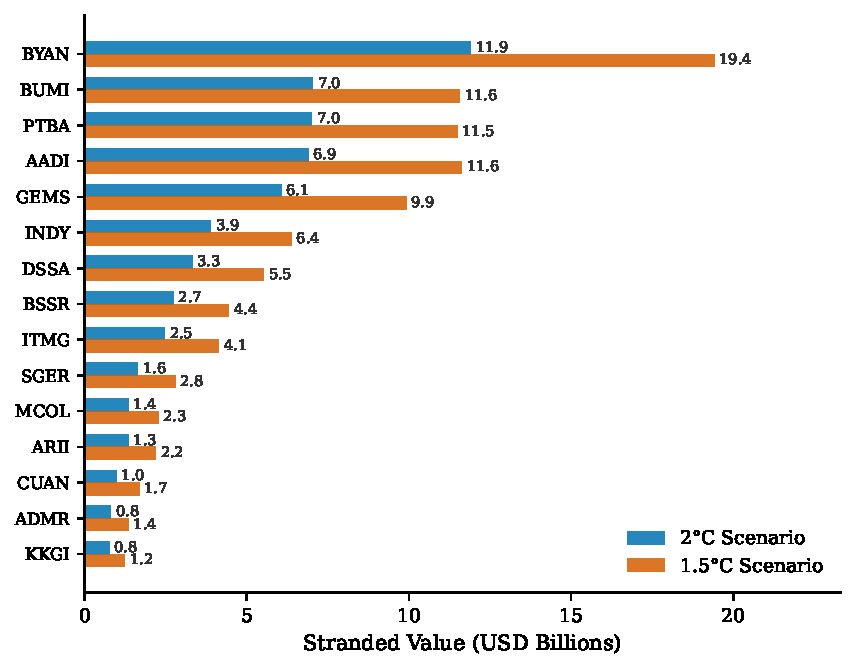
\includegraphics[width=\textwidth]{figures/fig_03.pdf}
\caption{Firm-level stranded values for the top 15 Indonesian coal companies under 2\textdegree C and 1.5\textdegree C scenarios. Values in USD millions. Companies ranked by expected stranded value (probability-weighted average across scenarios).}
\label{fig:firm_sv}
\end{figure}

\subsubsection{Policy Interpretation of the Supply Cost Curve}

The supply cost curve in Figure~\ref{fig:supply_cost} carries direct implications for just-transition policy design. Companies positioned above the 2\textdegree C price line (\$90/tonne at 2030) --- ITMG, TOBA, and HRUM --- are candidates for early operational restructuring rather than continued investment. These three companies together employ approximately 35,000 direct workers and support significant downstream logistics employment in East Kalimantan. A policy framework for managed coal phase-down that targets these companies first --- through negotiated early retirement packages, severance support, and mine rehabilitation financing --- would minimise the aggregate employment and fiscal impact while preserving the low-cost base of the sector for as long as a managed transition permits.

Conversely, the lowest-cost quartile --- BUMI, ADRO/AADI, and BYAN --- commands breakeven prices below \$60/tonne and therefore retains economic viability under even the 1.5\textdegree C scenario through the 2030 horizon. This heterogeneity suggests that a blanket moratorium on new coal investment is less efficient than a cost-based targeting approach, in which producers above the scenario-specific price line are denied new financing while those below the line are allowed to operate out their existing reserves under a strict no-new-expansion constraint. This distinction matters for bank lending policy: OJK could implement a tiered approach that restricts new lending to high-cost producers while allowing term loans to low-cost producers to continue under enhanced climate-risk disclosure and provisioning requirements.

\subsubsection{Probability-Weighted Expected Stranded Value and Investor Implications}

The probability-weighted expected stranded value of \$70.4 billion (90\% CI: \$59.7--82.1 billion) provides the most policy-relevant single estimate for investors pricing coal equity. This figure represents the actuarially fair discount that a rational investor should apply to the aggregate market value of Indonesia's listed coal sector, assuming that the three scenarios we consider span the relevant policy space and that our probability weights --- 30\% BAU, 40\% 2\textdegree C, 30\% 1.5\textdegree C --- are reasonable representations of the current policy distribution.

Notably, the aggregate market capitalisation of the 35 coal companies in our sample is approximately \$116 billion. The expected stranded value of \$70.4 billion represents approximately 61\% of this capitalisation, suggesting that Indonesian coal equities are substantially overvalued relative to a climate-adjusted fair value. This implies either that markets are assigning very high weight to the BAU scenario, that investors are discounting the probability of policy action, or that coal equity valuations are sustained by near-term earnings expectations rather than long-run reserve valuations. Our Monte Carlo uncertainty quantification allows us to construct a 90\% confidence interval for the market overvaluation: even in the most favourable scenario (the 5th percentile of expected stranded value, approximately \$52 billion), coal equities appear overvalued by roughly 45\% of current capitalisation. This finding is consistent with the broader international literature on carbon risk pricing \citep{BoltonKacperczyk2021} and reinforces the case for mandatory climate scenario disclosures that force markets to price transition risk more explicitly.

The comparison between the Monte Carlo uncertainty bounds and the scenario-specific point estimates is itself informative. The 90\% CI for the 2\textdegree C scenario (\$72.7--88.0 billion) reflects primarily parameter uncertainty within the scenario --- discount rates, cost growth, and production assumptions --- rather than cross-scenario uncertainty. The gap between the 2\textdegree C median (\$79.7 billion) and the 1.5\textdegree C median (\$128.3 billion) is therefore a better measure of the scenario risk faced by investors, while the confidence intervals around each estimate capture the econometric uncertainty in the methodology. Policymakers and investors should attend to both dimensions: our central estimates may be revised as better production and cost data become available, but the directional finding --- that Indonesian coal sector stranded values are large relative to bank equity and market capitalisation --- is robust across the full parameter space explored in our sensitivity analysis.



